% Provenance (never printed): see sources/outline_sources.md (Year 3: rift
% models, normal-fault systems, metamorphic core complexes, strike-slip
% systems). Brief: sources/book5/BRIEFS.md, ch. 9. Curves from
% figdata/bachelor-3/domino_extension.py and rollover.py. Exercise and problem
% values in the Book 5 scratch calculator calc/ch09.py.
\chapter{Tectónica extensional y de desgarre}\label{ch:b3:extension-strike-slip}

Entre la Sierra Nevada y la meseta del Colorado, las cordilleras y las cuencas
se alternan como los surcos de un campo, cada cordillera, un bloque de corteza basculado
a lo largo de una falla normal. En el núcleo de algunas de estas cordilleras, las rocas que habían estado
enterradas entre 23 y \qty{30}{km} de profundidad, a temperaturas de entre 500 y \qty{650}{\celsius}, hoy afloran en la
superficie, bajo una única falla que buza solo unos pocos grados.
Un continente puede estirarse en un factor de dos o más, y desgarrarse lateralmente a lo largo de fallas
que se curvan, escalonan y abren cuencas de hasta \qty{10}{km}. Este capítulo construye
la geometría de la extensión y del fallamiento de desgarre, las pocas reglas que
las gobiernan y las pruebas que dejan los sistemas reales.
% ledger: cooper10:snake-range, mcq05:basin-range, tb93:dead-sea-basin

\begin{recall}
Las fallas normales, de desgarre y transformantes, el semigraben y el rift continental
se estudian en el volumen de primer año, en sus capítulos sobre rifts y sobre fallas, pliegues
y fábricas, con la teoría de Anderson: con $\sigma_1$ vertical, las fallas normales
buzan $\ang{45} + \phi/2$, alrededor de \ang{60}; con $\sigma_2$ vertical, las
fallas de desgarre tienen rumbo a $\ang{45} - \phi/2$ respecto de $\sigma_1$. La ley de Byerlee sobre la
fricción de las rocas, $\tau = 0.85\,\sigma_n$ por debajo de \qty{200}{MPa} y $\tau =
\qty{50}{MPa} + 0.6\,\sigma_n$ por encima, se halla en su capítulo sobre esfuerzo, deformación y
reología. El modelo de estiramiento, en el que la litosfera se adelgaza de forma uniforme
por un factor $\beta$, y el modelo y la cuenca de rift se hallan en el volumen de segundo año, en su
capítulo dedicado a comparar cuencas sedimentarias. Las \omterm{def:b3:deformation-mechanisms:shear-zone}{zonas de cizalla} y las milonitas se encuentran en el
\cref{ch:b3:deformation-mechanisms}; la profundidad del despegue a partir del exceso
de área, $A = Sh$, en el \cref{ch:b3:structural-analysis}.
\end{recall}
% ledger: byerlee:1975

\section{Dos modelos de rift}\label{sec:b3:extension-strike-slip:models}

El modelo de estiramiento del volumen de segundo año adelgaza toda la litosfera por el
mismo factor bajo un mismo lugar: la corteza y el manto se adelgazan a la vez,
de forma simétrica, por cizalla pura. Muchos márgenes de rift no son simétricos: un lado
es una región amplia de bloques basculados, el otro una pendiente estrecha y empinada, y el
adelgazamiento del manto se sitúa al lado, y no debajo, del adelgazamiento de la corteza.

\begin{definition}[Modelo de rift por cizalla simple]\label{def:b3:extension-strike-slip:rift-models}
En el \emph{modelo de rift por cizalla simple}\index{modelo de rift por cizalla simple} la
litosfera se separa a lo largo de una \omterm{def:b3:deformation-mechanisms:shear-zone}{zona de cizalla} de bajo ángulo que la atraviesa
desde la superficie hasta su base. La placa situada sobre la \omterm{def:b3:deformation-mechanisms:shear-zone}{zona de cizalla}, la
placa superior, pierde su parte inferior; la placa de debajo, la placa inferior, es extraída
de debajo de ella. El adelgazamiento de la corteza y el del manto están
desplazados lateralmente, y los dos márgenes conjugados que se forman cuando el continente
se rompe son asimétricos.
\end{definition}

Los rifts reales combinan ambos: fallamiento frágil en la corteza superior, adelgazamiento dúctil
debajo, y un manto que puede adelgazarse en una región más amplia o más estrecha que la
corteza (estiramiento dependiente de la profundidad). Donde el manto caliente asciende bajo el
rift, o bajo su flanco en el caso de cizalla simple, la flotabilidad eleva los
bordes del rift, que se alzan como montañas sobre el fondo de la cuenca.

\begin{omfigure}
\begin{tikzpicture}[scale=0.95, >=stealth]
% (a) pure shear
\begin{scope}
\fill[omLithBasalt!40] (0,-3.2) rectangle (6.6,-1.3);
\fill[omLithGranite!50] (0,0) -- (2.2,0) -- (2.5,-0.35) -- (4.1,-0.35) -- (4.4,0) -- (6.6,0) -- (6.6,-1.3)
  -- (4.4,-1.3) -- (3.3,-0.95) -- (2.2,-1.3) -- (0,-1.3) -- cycle;
\fill[omLithBasalt!40] (2.2,-1.3) -- (3.3,-0.95) -- (4.4,-1.3) -- cycle;
\fill[orange!25] (0,-3.2) -- (1.8,-3.2) -- (3.3,-2.1) -- (4.8,-3.2) -- (6.6,-3.2) -- (6.6,-3.7) -- (0,-3.7) -- cycle;
\draw (0,0) -- (2.2,0) -- (2.5,-0.35) -- (4.1,-0.35) -- (4.4,0) -- (6.6,0);
\draw (0,-1.3) -- (2.2,-1.3) -- (3.3,-0.95) -- (4.4,-1.3) -- (6.6,-1.3);
\draw (0,-3.2) -- (1.8,-3.2) -- (3.3,-2.1) -- (4.8,-3.2) -- (6.6,-3.2);
\draw[thick] (2.2,0) -- (2.75,-0.85); \draw[thick] (4.4,0) -- (3.85,-0.85);
\node[font=\scriptsize] at (0.7,-0.65) {corteza};
\node[font=\scriptsize, align=center] at (0.9,-2.25) {manto\\ litosférico};
\node[font=\scriptsize] at (1.2,-3.48) {astenosfera};
\draw[<-] (-0.1,0.25) -- (0.6,0.25); \draw[->] (6.0,0.25) -- (6.7,0.25);
\node[font=\small] at (3.3,-4.2) {(a) cizalla pura};
\end{scope}
% (b) simple shear: crust thinned near the breakaway (left), mantle beneath the upper plate (right)
\begin{scope}[xshift=7.4cm]
\fill[omLithBasalt!40] (0,-3.2) rectangle (6.6,-1.3);
\fill[omLithGranite!50] (0,0) -- (0.9,0) -- (1.2,-0.3) -- (2.2,-0.3) -- (2.5,0) -- (4.0,0)
  .. controls (4.6,0.18) and (5.2,0.18) .. (5.8,0) -- (6.6,0) -- (6.6,-1.3)
  -- (2.9,-1.3) -- (2.0,-0.7) -- (1.2,-1.3) -- (0,-1.3) -- cycle;
\fill[omLithBasalt!40] (1.2,-1.3) -- (2.0,-0.7) -- (2.9,-1.3) -- cycle;
\fill[orange!25] (0,-3.2) -- (3.4,-3.2) -- (4.8,-2.1) -- (6.0,-3.2) -- (6.6,-3.2) -- (6.6,-3.7) -- (0,-3.7) -- cycle;
\draw (0,0) -- (0.9,0) -- (1.2,-0.3) -- (2.2,-0.3) -- (2.5,0) -- (4.0,0)
  .. controls (4.6,0.18) and (5.2,0.18) .. (5.8,0) -- (6.6,0);
\draw (0,-1.3) -- (1.2,-1.3) -- (2.0,-0.7) -- (2.9,-1.3) -- (6.6,-1.3);
\draw (0,-3.2) -- (3.4,-3.2) -- (4.8,-2.1) -- (6.0,-3.2) -- (6.6,-3.2);
\draw[omThm, very thick] (0.9,0) .. controls (2.4,-0.9) and (3.9,-1.8) .. (5.4,-3.2);
\node[font=\scriptsize, align=center] at (5.0,-0.6) {placa superior};
\node[font=\scriptsize, align=center] at (1.3,-2.3) {placa inferior};
\node[omThm, font=\scriptsize, align=center] at (3.0,-2.15) {zona de\\ cizalla};
\node[font=\scriptsize, align=center] at (4.9,0.42) {flanco levantado};
\draw[<-] (-0.1,0.25) -- (0.6,0.25); \draw[->] (6.0,0.25) -- (6.7,0.25);
\node[font=\small] at (3.3,-4.2) {(b) cizalla simple};
\end{scope}
\end{tikzpicture}

\par\smallskip{\small Dos modelos extremos de un rift (sin escala). (a) Cizalla
pura: la corteza y el manto litosférico se adelgazan juntos bajo el rift, con
fallas normales a ambos lados. (b) Cizalla simple: una \omterm{def:b3:deformation-mechanisms:shear-zone}{zona de cizalla} de bajo ángulo atraviesa
la litosfera; la corteza se adelgaza cerca de su traza superficial, el manto bajo
el lado opuesto, bajo la placa superior, de modo que el rift es asimétrico y su
flanco situado sobre el manto adelgazado está elevado.}\label{fig:b3:extension-strike-slip:models}
\end{omfigure}

\section{Sistemas de fallas normales}\label{sec:b3:extension-strike-slip:faults}

\begin{definition}[Fallas en dominó]\label{def:b3:extension-strike-slip:domino}
En las \emph{fallas en dominó}\index{fallas en dominó} un conjunto de
fallas normales planas y paralelas corta la corteza superior en bloques rígidos que, a medida que la región
se extiende, rotan a la vez como una hilera de libros que caen: las fallas se vuelven
menos empinadas y los estratos, inicialmente horizontales, se basculan en sentido contrario.
\end{definition}

\begin{theorem}[Extensión por dominós]\label{thm:b3:extension-strike-slip:domino}
Sean bloques rígidos limitados por fallas planas y paralelas que inicialmente buzan
$\theta_0$, y que rotan hasta que las fallas buzan $\theta$. Los estratos buzan entonces $\theta_0
- \theta$, alejándose de las fallas, y la región se ha extendido por el
factor
\[
  \beta = \frac{\sin\theta_0}{\sin\theta} .
\]
\end{theorem}

\begin{proof}
Los bloques son rígidos, por lo que la distancia perpendicular $d$ entre dos
fallas vecinas no cambia. A lo largo de una línea horizontal, dos planos paralelos
que buzan $\theta$ y distan $d$ entre sí cortan un segmento de longitud $d/\sin
\theta$; la anchura de la región varía como la longitud de ese segmento, desde
$d/\sin\theta_0$ hasta $d/\sin\theta$. Los bloques giran el ángulo en el que
se han aplanado las fallas, $\theta_0 - \theta$, y los estratos, horizontales,
al principio, giran con ellos.
\end{proof}

La rotación por sí sola produce una extensión moderada: fallas que parten de \ang{60} y
se aplanan hasta \ang{30} extienden la región en $\beta = 1.73$. No pueden rotar
indefinidamente: una falla se desliza cada vez con más dificultad a medida que se aplana, porque la
$\sigma_1$ vertical la oprime más y la cizalla menos.

\begin{proposition}[Bloqueo friccional de una falla normal]\label{prop:b3:extension-strike-slip:lockup}
Sea una falla sin cohesión con coeficiente de fricción $\mu$ que forma el ángulo
$t$ con $\sigma_1$, siendo todos los esfuerzos efectivos. Desliza cuando la razón de los
esfuerzos principales alcanza
\[
  \frac{\sigma_1}{\sigma_3} = \frac{1 + \mu\cot t}{1 - \mu\tan t} ,
\]
que es mínima, $(\sqrt{1 + \mu^2} + \mu)^2$, en $\tan2t = 1/\mu$, e
infinita en $\tan t = 1/\mu$. Con $\sigma_1$ vertical, el buzamiento de la falla es
$\ang{90} - t$: una falla normal que buza menos que $\arctan\mu$ no puede deslizar
en absoluto.
\end{proposition}

\begin{proof}
Se escriben $m = (\sigma_1 + \sigma_3)/2$ y $s = (\sigma_1 - \sigma_3)/2$. En
el plano, $\sigma_n = \sigma_1\sin^2t + \sigma_3\cos^2t = m - s\cos2t$ y
$\tau = (\sigma_1 - \sigma_3)\sin t\cos t = s\sin2t$. El deslizamiento exige $\tau =
\mu\sigma_n$; al dividir entre $\sigma_3\sin t\cos t$ y agrupar términos en $\sigma_1$
se obtiene la razón, cuyo denominador se anula en $\tan t = 1/\mu$. En la otra
forma, la condición se escribe $s(\sin2t + \mu\cos2t) = \mu m$. El paréntesis es como
máximo $\sqrt{1 + \mu^2}$, alcanzado en $\tan2t = 1/\mu$, donde el deslizamiento exige el
menor valor de $s/m = \mu/\sqrt{1 + \mu^2}$; entonces $\sigma_1/\sigma_3 = (m + s)/(m - s) =
(\sqrt{1 + \mu^2} + \mu)/(\sqrt{1 + \mu^2} - \mu) = (\sqrt{1 + \mu^2} +
\mu)^2$, puesto que el producto de los dos últimos paréntesis es 1.
\end{proof}

Con $\mu = 0.6$ de Byerlee, la falla normal mejor orientada buza \ang{60.5} y
desliza cuando $\sigma_1 = 3.12\,\sigma_3$; una falla a \ang{45} necesita $4.0$, y
ninguna que buza menos de \ang{31} desliza; con $\mu = 0.85$ el buzamiento de bloqueo es
\ang{40}. La figura siguiente muestra ambos resultados. Cuando un conjunto de dominós se acerca al
bloqueo, un nuevo conjunto de fallas empinadas corta al anterior: las regiones muy extendidas
muestran varias generaciones de fallas.

\begin{omfigure}
\begin{tikzpicture}
\begin{groupplot}[group style={group size=2 by 1, horizontal sep=1.6cm},
  omrecord, width=0.47\linewidth, height=0.42\linewidth, title style={font=\small},
  legend style={font=\scriptsize, legend cell align=left}]
\nextgroupplot[title={(a) extensión por dominós rígidos}, xlabel={buzamiento actual de la falla $\theta$ (\unit{\degree})},
  ylabel={factor de extensión $\beta$}, xmin=10, xmax=70, ymin=1, ymax=4,
  legend style={at={(0.97,0.97)}, anchor=north east}]
% computed in figdata/bachelor-3/domino_extension.py
\addplot[omDef, thick] table[x=dip, y=b70] {figdata/out/bachelor-3-domino_extension-beta.dat};
\addlegendentry{$\theta_0 = \ang{70}$}
\addplot[red!70!black, thick, densely dashed] table[x=dip, y=b60] {figdata/out/bachelor-3-domino_extension-beta.dat};
\addlegendentry{$\theta_0 = \ang{60}$}
\addplot[black, thick, densely dotted] table[x=dip, y=b45] {figdata/out/bachelor-3-domino_extension-beta.dat};
\addlegendentry{$\theta_0 = \ang{45}$}
\nextgroupplot[title={(b) razón de esfuerzos necesaria para el deslizamiento}, xlabel={buzamiento de la falla (\unit{\degree})},
  ylabel={$\sigma_1/\sigma_3$}, xmin=20, xmax=90, ymode=log, ymin=1, ymax=40,
  log ticks with fixed point, ytick={1,2,5,10,20,40},
  legend style={at={(0.97,0.97)}, anchor=north east}]
\addplot[omDef, thick] table[x=dip, y=r060] {figdata/out/bachelor-3-domino_extension-lockup.dat};
\addlegendentry{$\mu = 0.6$}
\addplot[red!70!black, thick, densely dashed] table[x=dip, y=r085] {figdata/out/bachelor-3-domino_extension-lockup.dat};
\addlegendentry{$\mu = 0.85$}
\end{groupplot}
\end{tikzpicture}

\par\smallskip{\small (a) Factor de extensión de un dominio de dominós rígidos conforme
sus fallas rotan desde el buzamiento inicial $\theta_0$ hasta $\theta$. (b) Razón de los
esfuerzos efectivos principales necesarios para deslizar una falla normal de un buzamiento dado
bajo un $\sigma_1$ vertical, para los dos coeficientes de fricción de Byerlee: mínima
cerca de \ang{60} y \ang{65}, e infinita en los buzamientos de bloqueo \ang{31} y
\ang{40}.}\label{fig:b3:extension-strike-slip:domino}
\end{omfigure}

Muchas fallas normales grandes son curvas, empinadas en la superficie y aplanadas en
profundidad hasta convertirse en una falla casi horizontal o en una \omterm{def:b3:deformation-mechanisms:shear-zone}{zona de cizalla}.

\begin{definition}[Falla de despegue, falla lístrica, anticlinal de rollover]\label{def:b3:extension-strike-slip:detachment}
Una \emph{falla de despegue}\index{falla de despegue} es una falla normal de bajo ángulo
o \omterm{def:b3:deformation-mechanisms:shear-zone}{zona de cizalla} de gran desplazamiento, de kilómetros a decenas de kilómetros, que
separa una placa superior extendida de una placa inferior deformada de forma distinta. Una
\emph{falla lístrica}\index{falla lístrica} es una falla normal cuyo buzamiento
disminuye con la profundidad, con un perfil cóncavo hacia arriba. Conforme el bloque superior
de una falla lístrica desciende y se aleja, se curva para mantenerse en contacto con la
falla: sus estratos se inclinan hacia ella formando un pliegue amplio, el \emph{anticlinal de
rollover}\index{anticlinal de rollover}.
\end{definition}

\begin{method}[La construcción de salto horizontal constante]\label{met:b3:extension-strike-slip:heave}
Para dibujar el bloque superior de una \omterm{def:b3:extension-strike-slip:detachment}{falla lístrica} tras un desplazamiento horizontal
$H$, el salto horizontal, en una sección paralela al deslizamiento:
\begin{enumerate}
  \item Se divide el bloque superior en columnas verticales. Cada columna se desplaza
        lateralmente una distancia $H$, alejándola del bloque inferior.
  \item Cada columna desciende en la caída de la falla que tiene debajo: una columna que
        parte donde la falla se encuentra a la profundidad $f(x)$ y termina donde se encuentra
        a $f(x + H)$ desciende $f(x + H) - f(x)$, lo que devuelve su base
        sobre la falla.
  \item El espacio que queda entre el bloque inferior y el bloque superior desplazado es el
        semigraben, que se rellena a medida que se abre con sedimentos que engrosan hacia la
        falla.
\end{enumerate}
Leída al revés, la construcción restaura la sección y predice la forma
de la falla a partir de la forma del rollover.
\end{method}

El área por debajo del nivel original de una capa, contada desde la falla, es
el área del \cref{ch:b3:structural-analysis} con el signo cambiado: $A =
H(D - z_0)$ para una capa situada inicialmente a la profundidad $z_0$ sobre un despegue
a la profundidad $D$, ya que la roca bajo la capa conserva su área mientras que su longitud aumenta
en $H$. Medir $A$ y $H$ en una sección sísmica permite obtener la profundidad del
despegue. La figura siguiente dibuja la construcción.

\begin{omfigure}
\begin{tikzpicture}
\begin{axis}[width=0.9\linewidth, height=0.36\linewidth, omsection,
  xmin=-2, xmax=24, ymin=0, ymax=6, y dir=reverse,
  xlabel={distancia (\unit{km})}, ylabel={profundidad (\unit{km})},
  legend style={font=\scriptsize, legend cell align=left, at={(0.98,0.27)}, anchor=south east}]
% computed in figdata/bachelor-3/rollover.py (heave 2 km, detachment at 5 km)
\addplot[name path=fault, black, very thick] table[x=x, y=z] {figdata/out/bachelor-3-rollover-fault.dat};
\addlegendentry{falla lístrica}
\addplot[name path=top, omDef, thick] table[x=x, y=z] {figdata/out/bachelor-3-rollover-top.dat};
\addlegendentry{techo del bloque superior}
\addplot[omDef, thick, densely dashed] table[x=x, y=z] {figdata/out/bachelor-3-rollover-bed.dat};
\addlegendentry{una capa situada inicialmente a \qty{2}{km}}
\addplot[gray, dashed, forget plot] coordinates {(-2,0) (24,0)};
\addplot[gray, dashed, forget plot] coordinates {(-2,5) (24,5)};
\node[font=\scriptsize, anchor=west] at (axis cs:15,5.35) {despegue};
\node[font=\scriptsize] at (axis cs:3.9,0.45) {semigraben};
\node[font=\scriptsize] at (axis cs:-1,1.5) {bloque inferior};
\node[font=\scriptsize] at (axis cs:9.5,1.15) {rollover};
\end{axis}
\end{tikzpicture}

\par\smallskip{\small \omterm{def:b3:extension-strike-slip:detachment}{Falla lístrica} que buza \ang{60} en superficie y se aplana
en un despegue a \qty{5}{km}, tras un salto horizontal de \qty{2}{km}
dibujado mediante la construcción de salto constante. El techo del bloque superior y una
capa más profunda se hunden hacia la falla formando un rollover; el área por debajo del techo
original, \qty{10}{km^2}, es el salto por la profundidad del despegue, y por debajo de
la capa más profunda, \qty{6}{km^2}, el salto por su altura sobre ella.}\label{fig:b3:extension-strike-slip:rollover}
\end{omfigure}

Las fallas normales no son infinitas. Cuando una falla se extingue a lo largo del rumbo,
su desplazamiento pasa a otra, que a menudo buza en sentido contrario, y los
semigrábenes de un rift se alternan en polaridad a lo largo de su longitud.

\begin{definition}[Zona de transferencia]\label{def:b3:extension-strike-slip:transfer}
Una \emph{zona de transferencia}\index{zona de transferencia} es la región comprendida entre dos
segmentos de falla normal, o segmentos de rift, que se solapan o están desplazados, a través de la cual
la extensión pasa de uno al otro: una rampa de relevo entre dos fallas
de la misma polaridad, un alto entre semigrábenes de polaridad opuesta, o una
falla de desgarre, la falla de transferencia, paralela a la extensión.
\end{definition}

\section{Complejos metamórficos de núcleo}\label{sec:b3:extension-strike-slip:core}

\begin{definition}[Complejo metamórfico de núcleo, charnela rodante]\label{def:b3:extension-strike-slip:core-complex}
Un \emph{complejo metamórfico de núcleo}\index{complejo metamórfico de núcleo} es una cúpula de
rocas metamórficas y milonitas, elevada desde la corteza media o inferior,
bajo una \omterm{def:b3:extension-strike-slip:detachment}{falla de despegue} cuyo bloque superior es un mosaico de bloques basculados de
rocas de la corteza superior. En el modelo de \emph{charnela rodante}\index{charnela rodante},
el despegue desliza con un buzamiento moderado en profundidad; a medida que el bloque superior
se aleja, el bloque inferior descargado se eleva por isostasia y se curva, de modo que cada parte
de la falla rota hasta un buzamiento bajo y deja de deslizar una vez que ha pasado
por una charnela que migra con la extensión.
\end{definition}

Las milonitas del bloque inferior registran la parte profunda de la historia: son la
\omterm{def:b3:deformation-mechanisms:shear-zone}{zona de cizalla} del \cref{ch:b3:deformation-mechanisms}, y sus \omterm{def:b3:deformation-mechanisms:kinematic}{indicadores
cinemáticos} dan el sentido de transporte del bloque superior. Más arriba, las
mismas rocas atraviesan la transición frágil--dúctil y quedan sobreimpresas por
cataclasitas y brechas justo bajo la falla. En la sierra Snake del norte de Nevada, los
esquistos con granate del bloque inferior alcanzaron de 6 a \qty{8}{kbar} y
de 500 a \qty{650}{\celsius}, profundidades de enterramiento de 23 a \qty{30}{km}; el
despegue que los elevó se interpreta como una \omterm{def:b3:extension-strike-slip:core-complex}{charnela rodante}.
% ledger: cooper10:snake-range

\begin{omfigure}
\begin{tikzpicture}[scale=1.0, >=stealth]
% upper plate dominoes on the left
\foreach \x in {0.0,0.9,1.8} {
  \fill[omLithSand] (\x,0) -- (\x+0.8,0) -- (\x+1.3,-0.9+0.25*\x) -- (\x+0.4,-1.5+0.2*\x) -- cycle;
  \draw (\x,0) -- (\x+0.8,0) -- (\x+1.3,-0.9+0.25*\x) -- (\x+0.4,-1.5+0.2*\x) -- cycle;
}
\fill[omLithGranite!45] (0,-2.6) -- (0,-1.6) .. controls (2.5,-1.2) and (4.0,-0.15) .. (6.0,-0.1)
  .. controls (8.0,-0.15) and (9.5,-0.9) .. (11.2,-1.0) -- (11.2,-2.6) -- cycle;
\fill[pattern=horizontal lines, pattern color=gray] (0,-1.6) .. controls (2.5,-1.2) and (4.0,-0.15) .. (6.0,-0.1)
  .. controls (8.0,-0.15) and (9.5,-0.9) .. (11.2,-1.0) -- (11.2,-1.35)
  .. controls (9.5,-1.25) and (8.0,-0.5) .. (6.0,-0.45) .. controls (4.0,-0.5) and (2.5,-1.55) .. (0,-1.95) -- cycle;
\draw[omThm, very thick] (0,-1.6) .. controls (2.5,-1.2) and (4.0,-0.15) .. (6.0,-0.1)
  .. controls (8.0,-0.15) and (9.5,-0.9) .. (11.2,-1.0);
% upper plate to the right, still in place
\fill[omLithSand] (8.4,0) -- (11.2,0) -- (11.2,-1.0) .. controls (10.2,-0.95) and (9.3,-0.75) .. (8.4,-0.35) -- cycle;
\draw (8.4,0) -- (11.2,0); \draw (8.4,0) -- (8.4,-0.35);
\node[font=\scriptsize] at (9.9,-0.45) {bloque superior};
\node[font=\scriptsize] at (1.5,0.3) {bloques basculados};
\node[omThm, font=\scriptsize] at (6.0,0.15) {despegue};
\node[font=\scriptsize] at (6.0,-0.75) {milonitas};
\node[font=\scriptsize, align=center] at (6.0,-1.8) {bloque inferior de\\ corteza media};
\draw[->, thick] (6.0,-2.9) -- (6.0,-2.2) node[pos=0, below, font=\scriptsize] {ascenso isostático};
\draw[->, omThm] (10.4,0.3) -- (11.1,0.3);
\draw[->, omThm] (1.0,0.55) -- (0.3,0.55);
\draw[dashed] (7.6,-0.3) -- (8.6,-1.5) node[below, font=\scriptsize] {charnela rodante};
\end{tikzpicture}

\par\smallskip{\small Anatomía de un \omterm{def:b3:extension-strike-slip:core-complex}{complejo metamórfico de núcleo} (no a escala).
El bloque inferior, situado bajo el despegue, es una cúpula de rocas de corteza media con una
coraza de milonitas, se eleva bajo el bloque superior a medida que este se separa
hacia ambos lados; la parte del despegue que ha pasado la \omterm{def:b3:extension-strike-slip:core-complex}{charnela rodante}
se ha curvado hasta un buzamiento bajo y ya no desliza. Los bloques basculados del
bloque superior descansan sobre el despegue.}\label{fig:b3:extension-strike-slip:core}
\end{omfigure}

Los buzamientos bajos son una paradoja: según la proposición de bloqueo, ninguna falla normal
que buza menos de unos \ang{31} debería deslizar bajo un $\sigma_1$ vertical
con la fricción de Byerlee. La \omterm{def:b3:extension-strike-slip:core-complex}{charnela rodante} es una salida: la parte activa de la
falla es más empinada de lo que se observa. Las otras son una falla debilitada por arcillas
o por fluidos a alta presión, lo que reduce el $\mu$ efectivo, o un campo de
esfuerzos rotado cerca de una \omterm{def:b3:deformation-mechanisms:shear-zone}{zona de cizalla} en profundidad; los terremotos en fallas normales de bajo ángulo
son raros, lo que favorece que deslicen mientras siguen empinadas o que deslicen sin terremotos.

\section{Sistemas de desgarre}\label{sec:b3:extension-strike-slip:strike-slip}

En los experimentos con pasta de arcilla y en la naturaleza, una falla de desgarre no corta un
plano limpio a través de una cobertera de sedimentos: crece como una banda de fracturas cortas,
en échelon, con ángulos constantes.

\begin{definition}[Cizalla de Riedel]\label{def:b3:extension-strike-slip:riedel}
En una \omterm{def:b3:deformation-mechanisms:shear-zone}{zona de cizalla} simple de desgarre, \emph{cizallas de Riedel}\index{cizallas de Riedel}
son las fracturas de cizalla cortas que se forman primero, en dos conjuntos: las cizallas R,
con un ángulo pequeño respecto a la zona y con su sentido de deslizamiento, y las cizallas R$'$,
con un ángulo grande y con el sentido opuesto. Más tarde, las cizallas P, simétricas
a las R respecto a la zona, y las fracturas de tensión T completan el patrón.
\end{definition}

\begin{proposition}[Ángulos de Riedel]\label{prop:b3:extension-strike-slip:riedel}
En una \omterm{def:b3:deformation-mechanisms:shear-zone}{zona de cizalla} simple, $\sigma_1$ yace en el plano horizontal formando
\ang{45} con la zona. Para una roca que rompe según el criterio de Coulomb con el
ángulo de fricción interna $\phi$, las cizallas R forman con la zona el ángulo $\phi/2$, y las
cizallas R$'$ forman $\ang{90} - \phi/2$, ambos medidos desde la zona
por el lado de $\sigma_1$, y las fracturas de tensión se forman paralelas a $\sigma_1$,
a \ang{45}.
\end{proposition}

\begin{proof}
En la cizalla simple, las direcciones principales de la deformación infinitesimal están a
\ang{45} del plano de cizalla, y un material isótropo se carga con
$\sigma_1$ según la dirección de acortamiento. Por el teorema de Anderson, los dos planos de Coulomb
contienen a $\sigma_2$, vertical aquí, y forman $\ang{45} - \phi/2$ con
$\sigma_1$ a cada lado: el más próximo a la zona a $\ang{45} -
(\ang{45} - \phi/2) = \phi/2$ de ella, el otro a $\ang{45} + \ang{45} -
\phi/2$. Cada uno desliza de forma que acorta según $\sigma_1$: la cizalla R con
la zona, la cizalla R$'$ en sentido contrario. Las fracturas de tensión se abren frente a $\sigma_3$ y
son perpendiculares a él.
\end{proof}

Con $\phi = \ang{30}$, las cizallas R quedan a \ang{15} y las cizallas R$'$ a
\ang{75}. Cuando la falla principal no es recta, los bloques a ambos lados
convergen o divergen a través de ella.

\begin{definition}[Curvatura contractiva, curvatura distensiva]\label{def:b3:extension-strike-slip:bends}
Una curvatura o escalón en una falla de desgarre es una \emph{curvatura
contractiva}\index{curvatura contractiva} cuando el movimiento de los bloques los empuja uno contra otro
a través de ella, y una \emph{curvatura distensiva}\index{curvatura distensiva} cuando los separa. Para una falla
dextral, un escalón hacia la derecha es distensivo y uno hacia la izquierda contractivo;
en una falla sinistral, lo contrario.
\end{definition}

\begin{definition}[Cuenca de pull-apart]\label{def:b3:extension-strike-slip:pull-apart}
Una \emph{cuenca de pull-apart}\index{cuenca de pull-apart} es una cuenca que se abre en
un escalón distensivo entre dos segmentos de falla de desgarre que se solapan, limitada por
los segmentos a lo largo de sus lados largos y por fallas normales oblicuas en sus extremos.
Su área crece como el producto de la anchura del escalón por el desplazamiento de la falla.
\end{definition}

\begin{definition}[Estructura en flor]\label{def:b3:extension-strike-slip:flower}
Una \emph{estructura en flor}\index{estructura en flor} es el abanico de ramales de falla,
visto en una sección transversal, en el que una falla de desgarre empinada se divide al acercarse a la
superficie: una flor positiva, cuyos ramales tienen componente inversa
y levantan una cresta, en una \omterm{def:b3:extension-strike-slip:bends}{curvatura contractiva}; una flor negativa, cuyos ramales tienen
componente normal y encuadran una depresión, en una \omterm{def:b3:extension-strike-slip:bends}{curvatura distensiva}.
\end{definition}

\begin{definition}[Transpresión, transtensión]\label{def:b3:extension-strike-slip:transpression}
La \emph{transpresión}\index{transpresión} es la deformación de desgarre combinada
con acortamiento a través de la zona; la \emph{transtensión}\index{transtensión},
la deformación de desgarre combinada con extensión a través de ella. Ambas aparecen donde
el movimiento entre dos bloques es oblicuo al límite que los separa.
\end{definition}

El movimiento oblicuo suele estar repartido: una falla de desgarre toma el movimiento
paralelo al límite, y cabalgamientos o pliegues junto a ella, o fallas normales, toman el movimiento
a través de él.

\begin{omfigure}
\begin{tikzpicture}[scale=1.0, >=stealth]
% (a) Riedel geometry, dextral E-W zone
\begin{scope}
\draw[thick] (0,0.9) -- (5,0.9); \draw[thick] (0,-0.9) -- (5,-0.9);
\draw[->] (1.0,1.15) -- (2.0,1.15); \draw[->] (4.0,-1.15) -- (3.0,-1.15);
\foreach \x in {0.6,1.6,2.6,3.6} \draw[omDef, thick] (\x,0.2) -- ++(-15:0.9);
\node[omDef, font=\scriptsize] at (4.6,0.05) {R};
\foreach \x in {1.0,2.4} \draw[red!70!black, thick] (\x,-0.6) -- ++(105:0.75);
\node[red!70!black, font=\scriptsize] at (1.0,-0.75) {R$'$};
\foreach \x in {3.3,3.7,4.1} \draw[black, thick] (\x,-0.25) -- ++(15:0.45);
\node[font=\scriptsize] at (4.6,-0.35) {P};
\foreach \x in {0.5,0.9} \draw[omMeth, line width=1.4pt] (\x,0.45) -- ++(135:0.35);
\node[omMeth, font=\scriptsize] at (0.25,0.25) {T};
\draw[<->, omThm] ($(2.6,0)+(135:0.55)$) -- ($(2.6,0)+(-45:0.55)$);
\node[omThm, font=\scriptsize] at (2.05,0.62) {$\sigma_1$};
\node[font=\small] at (2.5,-1.6) {(a) cizallas de Riedel, dextral};
\end{scope}
% (b) releasing and restraining steps on a dextral fault
\begin{scope}[xshift=6.0cm]
\fill[omLithSand!70] (1.6,0.75) -- (2.6,0.75) -- (2.6,0.25) -- (1.6,0.25) -- cycle;
\draw[thick] (0,0.75) -- (2.6,0.75); \draw[thick] (1.6,0.25) -- (4.2,0.25);
\draw[->] (0.3,1.0) -- (1.0,1.0); \draw[->] (3.9,0.0) -- (3.2,0.0);
\node[font=\scriptsize] at (2.1,0.5) {cuenca};
\node[font=\scriptsize, anchor=west] at (2.75,0.95) {distensiva};
\fill[omLithGranite!60] (1.6,-0.65) -- (2.6,-0.65) -- (2.6,-1.15) -- (1.6,-1.15) -- cycle;
\draw[thick] (0,-1.15) -- (2.6,-1.15); \draw[thick] (1.6,-0.65) -- (4.2,-0.65);
\draw[->] (0.3,-0.9) -- (1.0,-0.9); \draw[->] (3.9,-0.9) -- (3.2,-0.9);
\node[font=\scriptsize] at (2.1,-0.9) {cresta};
\node[font=\scriptsize, anchor=west] at (2.75,-0.45) {contractiva};
\node[font=\small] at (2.1,-1.6) {(b) escalones, dextral, en planta};
\end{scope}
% (c) flower structures in section
\begin{scope}[xshift=11.0cm]
\draw[thick] (1.0,-1.3) -- (1.0,-0.4);
\draw[thick] (1.0,-0.4) .. controls (0.9,0.1) .. (0.45,0.8);
\draw[thick] (1.0,-0.4) -- (1.0,0.8);
\draw[thick] (1.0,-0.4) .. controls (1.1,0.1) .. (1.55,0.8);
\draw (0.0,0.8) -- (0.45,0.8) .. controls (0.8,1.1) and (1.2,1.1) .. (1.55,0.8) -- (2.0,0.8);
\node[font=\scriptsize, align=center] at (1.0,-1.6) {positiva};
\draw[thick] (3.2,-1.3) -- (3.2,-0.4);
\draw[thick] (3.2,-0.4) .. controls (3.1,0.1) .. (2.65,0.8);
\draw[thick] (3.2,-0.4) -- (3.2,0.8);
\draw[thick] (3.2,-0.4) .. controls (3.3,0.1) .. (3.75,0.8);
\draw (2.2,0.8) -- (2.65,0.8) .. controls (3.0,0.5) and (3.4,0.5) .. (3.75,0.8) -- (4.2,0.8);
\node[font=\scriptsize, align=center] at (3.2,-1.6) {negativa};
\node[font=\small] at (2.1,-1.95) {(c) flores, sección};
\end{scope}
\end{tikzpicture}

\par\smallskip{\small Estructuras de desgarre (no a escala). (a) En una zona dextral,
$\sigma_1$ a \ang{45}: cizallas R a \ang{15} y cizallas P a
\ang{-15} con el sentido de la zona, cizallas R$'$ a \ang{75} con el sentido
opuesto, fracturas de tracción T paralelas a $\sigma_1$. (b) Un escalón
hacia la derecha en una falla dextral abre una \omterm{def:b3:extension-strike-slip:pull-apart}{cuenca de pull-apart}; un
escalón hacia la izquierda empuja hacia arriba una cresta. (c) La falla se
ramifica hacia arriba formando una \omterm{def:b3:extension-strike-slip:flower}{estructura en flor} positiva bajo una cresta y una \omterm{def:b3:extension-strike-slip:flower}{estructura en flor} negativa bajo una depresión.}\label{fig:b3:extension-strike-slip:strike-slip}
\end{omfigure}

\section{Tres sistemas}\label{sec:b3:extension-strike-slip:systems}

\paragraph{La Cuenca y Cordillera.} Una reconstrucción de la región desde
hace \qty{36}{Ma} encuentra unos \qty{235}{km} de extensión, orientada hacia
N\ang{78}O, tanto en el norte, donde alcanza el \qty{50}{\percent}, como en
el centro, donde llega al \qty{200}{\percent}: la parte central es tres
veces más ancha que antes. Desde hace entre 10 y \qty{12}{Ma}, parte del
movimiento dextral del límite entre el Pacífico y Norteamérica ha saltado al
continente, unos \qty{100}{km} orientados hacia N\ang{25}O, a unos
\qty{1}{cm/yr}: la región es ahora transtensional. Sus complejos de núcleo se sitúan donde la extensión fue mayor.
% ledger: mcq05:basin-range

\paragraph{El mar Muerto.} La Transformante del mar Muerto ha acumulado unos
\qty{105}{km} de movimiento sinistral entre África y Arabia desde hace unos
\qty{20}{Ma}. A lo largo de ella, la cuenca del mar Muerto es un pull-apart de
\qty{132}{km} de longitud, de 7 a \qty{10}{km} de anchura y de hasta
\qty{10}{km} de profundidad, delimitada en sus flancos por fallas
subverticales; los modelos gravimétricos dan \qty{21}{km} de estiramiento a
lo largo de su eje, un factor de 1.19, que a la velocidad de placa de
\qty{6}{mm/yr} requiere unos \qty{3.5}{Myr}. En otros puntos de la
transformante, un segmento muestra una \omterm{def:b3:extension-strike-slip:flower}{estructura en flor} positiva de 100 a \qty{300}{m} de anchura en sus primeros pocos cientos de metros superiores, y otros son pequeños pull-aparts.
% ledger: weber09:dst, tb93:dead-sea-basin

\paragraph{La falla de San Andrés.} El sistema de fallas tiene más de
\qty{1290}{km} (800 millas) de longitud; ha desplazado al menos
\qty{560}{km} (350 millas) desde que se formó hace entre 15 y \qty{20}{Ma}, y
la medición muestra una deriva de hasta unos \qty{5}{cm/yr} (2 pulgadas
al año). Donde se curva hacia el norte de Los Ángeles, el movimiento es
oblicuo a la falla: los bloques situados dentro y junto a la zona de falla en
las montañas de San Bernardino se han elevado entre 3 y \qty{4}{km} o más, a
\qty{1.5}{mm/yr} o más, por la convergencia y la partición del deslizamiento de la \omterm{def:b3:extension-strike-slip:transpression}{transpresión}.
% ledger: usgs:saf, sp98:san-bernardino

\begin{inthefield}[Cartografía de una falla de despegue]
\begin{minipage}[t]{0.55\linewidth}\vspace{0pt}
En un complejo de núcleo, el despegue forma a menudo la superficie suave y de
buzamiento suave de la propia sierra, donde la erosión ha desmantelado el
bloque superior. Los geólogos que la cartografían siguen el contacto entre
las rocas frágiles del bloque superior y las milonitas inferiores, representan
su actitud cada pocos cientos de metros en un estereograma y miden las
lineaciones de la superficie de falla y de las milonitas: su dirección indica
el sentido del transporte, y sus \omterm{def:b3:deformation-mechanisms:kinematic}{indicadores cinemáticos}, el sentido. Las
muestras del bloque inferior se llevan al laboratorio para geobarometría y
para edades minerales que datan su enfriamiento; los bloques superiores se
cartografían por la inclinación de sus capas, que registra cuánto han rotado sus fallas.
\end{minipage}\hfill
\begin{minipage}[t]{0.42\linewidth}\vspace{0pt}
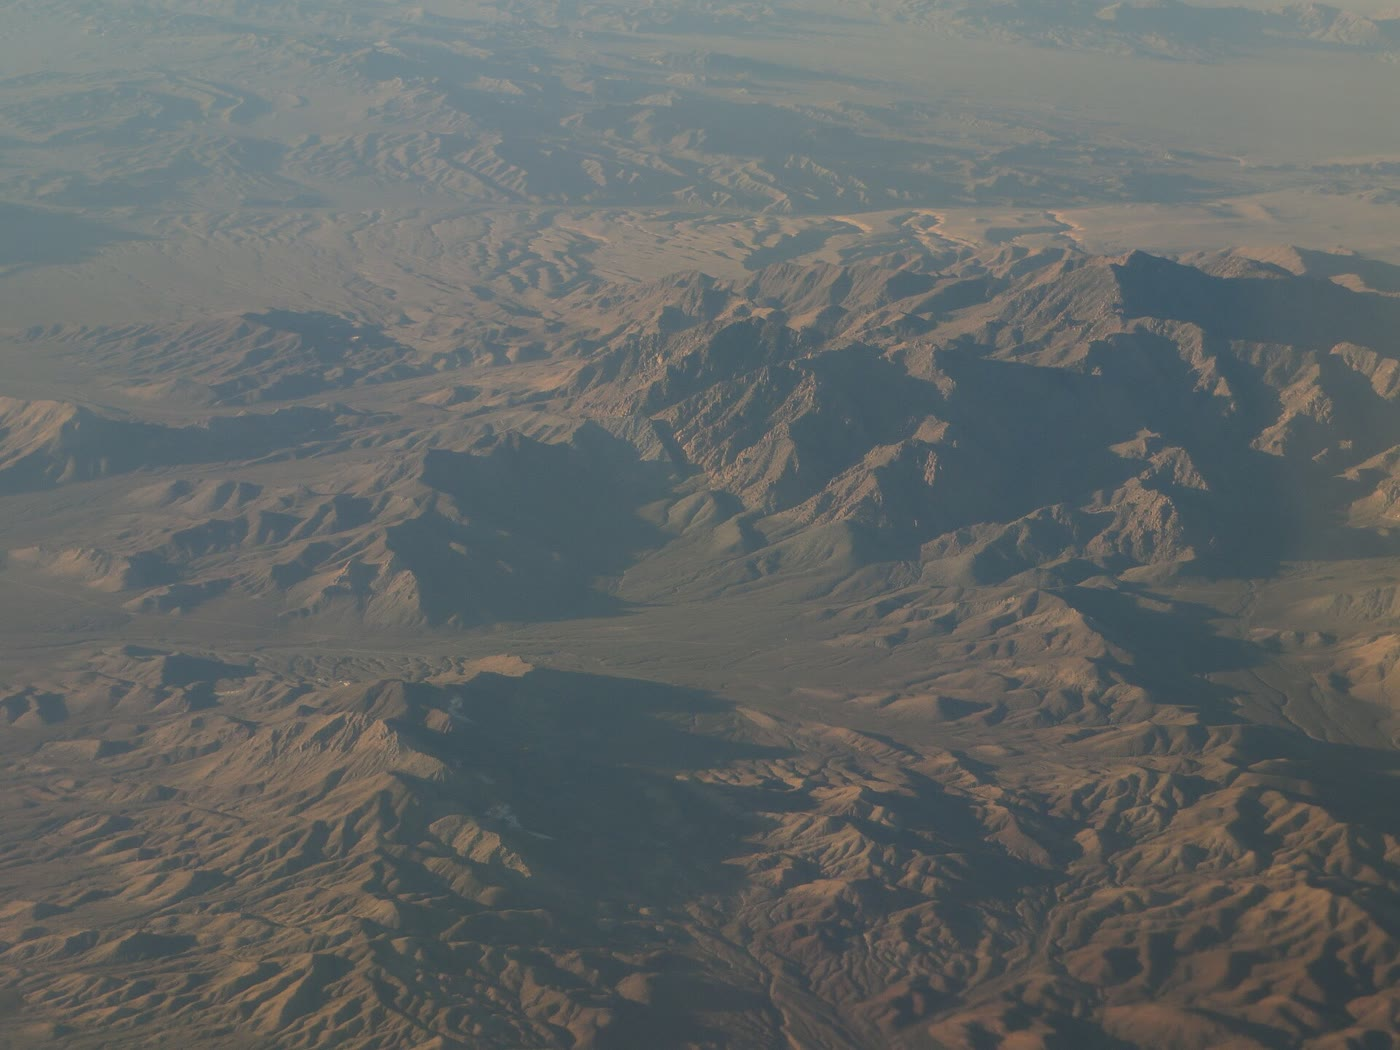
\includegraphics[width=\linewidth]{images/book5/b3-basin-and-range.jpg}

{\scriptsize Topografía de cuenca y cordillera al sur de Death Valley, California,
vista desde el aire: sierras paralelas de bloques de falla inclinados separados
por cuencas rellenas de sedimento. Foto Ken Lund, CC BY-SA 2.0.}
\end{minipage}
\end{inthefield}
% ledger: photo:b3-basin-and-range

\section{Ejercicios}

\begin{exercise}[$\star$]\label{exo:b3:extension-strike-slip:1}
Un dominio de bloques rígidos en dominó tiene fallas con buzamiento de \ang{35}; se formaron
a \ang{50}. Calcúlese el buzamiento de las capas y el factor de extensión.
\end{exercise}

\begin{exercise}[$\star$]\label{exo:b3:extension-strike-slip:2}
Indíquese si cada escalón abre una cuenca o levanta una cresta: una falla
dextral con escalón hacia la derecha; una falla dextral con escalón hacia la
izquierda; una falla sinistral con escalón hacia la izquierda; una falla sinistral con escalón hacia la derecha.
\end{exercise}

\begin{exercise}[$\star$]\label{exo:b3:extension-strike-slip:3}
La Transformante del mar Muerto ha desplazado \qty{105}{km} en unos
\qty{20}{Myr}. Calcúlese la velocidad media en \unit{mm/yr} y compárese con los
\qty{6}{mm/yr} usados para la cuenca del mar Muerto.
\end{exercise}

\begin{exercise}[$\star$]\label{exo:b3:extension-strike-slip:4}
En el centro de la Cuenca y Cordillera, \qty{235}{km} de extensión equivalen
al \qty{200}{\percent}. Calcúlese la anchura de la región antes y después.
Háganse lo mismo para la parte norte, con el \qty{50}{\percent}.
\end{exercise}

\begin{exercise}[$\star\star$]\label{exo:b3:extension-strike-slip:5}
La falla de San Andrés ha desplazado al menos \qty{563}{km} en un intervalo de 15 a
\qty{20}{Myr}. Calcúlese el intervalo de velocidades medias y compárese con una
deriva actual de unos \qty{51}{mm/yr}. ¿Qué podría explicar la diferencia?
\end{exercise}

\begin{exercise}[$\star\star$]\label{exo:b3:extension-strike-slip:6}
Con $\mu = 0.6$, calcúlese la razón $\sigma_1/\sigma_3$ necesaria para deslizar
fallas normales con buzamiento de \ang{60}, \ang{50} y \ang{40}, y el buzamiento de bloqueo.
\end{exercise}

\begin{exercise}[$\star\star$]\label{exo:b3:extension-strike-slip:7}
Calcúlese el buzamiento de bloqueo de una falla normal para $\mu = 0.4$ y
$\mu = 0.2$. ¿Qué coeficiente de fricción permitiría que una falla con
buzamiento de \ang{15} deslizara bajo un $\sigma_1$ vertical?
\end{exercise}

\begin{exercise}[$\star\star$]\label{exo:b3:extension-strike-slip:8}
En una sección sísmica paralela al deslizamiento, una \omterm{def:b3:extension-strike-slip:detachment}{falla lístrica} tiene un salto horizontal de
\qty{2.5}{km}; se aplana en una \omterm{def:b3:extension-strike-slip:detachment}{falla de despegue} a \qty{4.0}{km} de profundidad. Calcúlese el área
de la depresión por debajo de la superficie original del bloque superior, y por debajo de una capa
situada primero a \qty{1.5}{km} de profundidad.
\end{exercise}

\begin{exercise}[$\star\star$]\label{exo:b3:extension-strike-slip:9}
La cuenca del Mar Muerto mide \qty{132}{km} de largo y se ha estirado por un factor de 1.19
a lo largo de su eje. Calcúlense su longitud inicial y el estiramiento, y el tiempo
que tarda en producirse ese estiramiento a \qty{6}{mm/yr}.
\end{exercise}

\begin{exercise}[$\star\star\star$]\label{exo:b3:extension-strike-slip:10}
Bloques separados \qty{3.0}{km}, medidos perpendicularmente a sus fallas, rotan
desde buzamientos de las fallas de \ang{60} hasta \ang{45}. Calcúlense la anchura horizontal de un
bloque antes y después, el estiramiento por bloque y el buzamiento de las capas.
¿Por qué las capas deben buzar en sentido contrario al de las fallas?
\end{exercise}

\begin{exercise}[$\star\star\star$]\label{exo:b3:extension-strike-slip:11}
Dénse los ángulos de las cizallas R y R$'$ y de las fracturas de tensión para una
roca con $\phi = \ang{40}$ en una zona sinestral de rumbo este--oeste, como
acimutes, y sus sentidos de deslizamiento.
\end{exercise}

\begin{exercise}[$\star\star\star$]\label{exo:b3:extension-strike-slip:12}
Un dominio de \omterm{def:b3:extension-strike-slip:domino}{fallas en dominó} se forma con sus fallas en el buzamiento óptimo para el deslizamiento y
rota hasta que se bloquean. Calcúlese el mayor factor de extensión que la rotación
por sí sola produce para $\mu = 0.6$ y para $\mu = 0.85$, e indíquense qué
rocas pueden estirarse más antes de que deban formarse nuevas fallas.
\end{exercise}

\section{Problema: el semigraben de Merrow}

\begin{problem}[{Problema de fin de semana --- la extensión de un borde de rift
inventado, a partir de sus fallas en dominó, su falla lístrica, su complejo de núcleo y su
falla de transferencia}]
\label{pb:b3:extension-strike-slip:1}
% values: calc/ch09.py; domino_extension.py; rollover.py
El semigraben de Merrow es una cuenca inventada en el borde de un rift continental
Su falla maestra es lístrica, con buzamiento de \ang{60} en superficie.
En su bloque superior, un dominio de \qty{24.0}{km} de anchura está cortado por fallas planas que hoy buzan
\ang{42} al E, entre las cuales las capas buzan \ang{18} al O. En una sección sísmica
paralela al deslizamiento, la falla maestra tiene un salto horizontal de \qty{3.2}{km} y la
parte superior de su bloque superior se deprime por debajo de su nivel original en un área de
\qty{16.0}{km^2}. A lo largo del rumbo hacia el sur, la erosión ha eliminado la
placa superior del mismo sistema y ha dejado al descubierto un complejo de núcleo. Hacia el norte, una
falla de transferencia sinestral une el semigraben con el siguiente. Tómense $\mu =
0.6$, $g = \qty{9.8}{m/s^2}$ y una densidad cortical de
\qty{2800}{kg/m^3}.

\medskip\noindent\textbf{Parte I --- Las fallas en dominó.}
\begin{enumerate}
  \item ¿Por qué el buzamiento inicial de las fallas es la suma del buzamiento actual de la falla y
        de las capas? Dése su valor y compárese con la teoría de Anderson.
  \item Calcúlese el factor de extensión del dominio.
  \item Calcúlense la anchura inicial del dominio y la extensión que registra.
  \item Calcúlese la razón $\sigma_1/\sigma_3$ necesaria para hacer deslizar ahora las fallas,
        y compárese con la de fallas nuevas, bien orientadas.
  \item ¿Con qué buzamiento se bloquean estas fallas, y qué factor de extensión podría
        alcanzar el dominio solo por rotación? ¿Qué ocurre entonces?
\end{enumerate}

\medskip\noindent\textbf{Parte II --- La falla maestra lístrica.}
\begin{enumerate}[resume]
  \item Explíquese, con la construcción de salto horizontal constante, por qué las capas del bloque superior
        se inclinan hacia la falla.
  \item Calcúlese la profundidad de la \omterm{def:b3:extension-strike-slip:detachment}{falla de despegue}.
  \item El área de la depresión se conoce con una precisión del \qty{10}{\percent}. ¿Cuán bien se conoce la
        profundidad?
  \item ¿Qué área de depresión se predice para una capa situada primero a \qty{2.0}{km}
        de profundidad?
  \item ¿Cuál es la extensión horizontal a través de la falla maestra?
  \item ¿Cómo registran los sedimentos del semigraben la actividad de la
        falla?
\end{enumerate}

\medskip\noindent\textbf{Parte III --- El complejo metamórfico de núcleo.}
\begin{enumerate}[resume]
  \item Las milonitas del bloque inferior se equilibraron a \qty{5.5}{kbar}. Calcúlese
        su profundidad.
  \item Sus micas se cerraron al argón a \qty{24}{Ma}, y los cantos de esas mismas
        milonitas aparecen en el relleno del semigraben a \qty{16}{Ma}. Calcúlese la tasa media de
        exhumación, tomando la profundidad de cierre como la profundidad de la
        pregunta anterior.
  \item Para llevar las milonitas a la superficie, ¿cuánto deslizamiento se necesita en una \omterm{def:b3:extension-strike-slip:detachment}{falla de
        despegue} de buzamiento medio de \ang{30}, y cuánta extensión horizontal?
  \item La \omterm{def:b3:extension-strike-slip:detachment}{falla de despegue} buza hoy \ang{15} en superficie. ¿Pudo haber
        deslizado con ese buzamiento bajo un $\sigma_1$ vertical? Indíquense dos salidas.
  \item Si deslizó a \ang{45} en profundidad, ¿en qué ángulo ha rotado la
        parte expuesta, y por qué?
  \item Compárese la extensión del complejo de núcleo con la del
        semigraben.
\end{enumerate}

\medskip\noindent\textbf{Parte IV --- La falla de transferencia.}
\begin{enumerate}[resume]
  \item La falla de transferencia sinestral presenta un escalón de \qty{4.0}{km} hacia la izquierda, con sus dos
        ramales solapándose a lo largo de \qty{3.0}{km}. ¿Abre el escalón una cuenca
        o eleva una cresta?
  \item La falla ha deslizado a \qty{5}{mm/yr} durante \qty{1.2}{Myr}. Calcúlese
        el desplazamiento.
  \item Calcúlense el área abierta, la longitud del fondo de la cuenca (solape más
        desplazamiento) y su razón entre longitud y anchura.
  \item Compárese esa razón con la de la cuenca del Mar Muerto, de \qty{132}{km} de longitud y de 7
        a \qty{10}{km} de anchura.
  \item Donde la misma falla se curva en sentido contrario, ¿qué estructura se forma, y
        qué mostraría una sección transversal a través de ella?
  \item ¿Cuál es la extensión horizontal total a través del semigraben de Merrow,
        a partir de su falla maestra y de sus \omterm{def:b3:extension-strike-slip:domino}{fallas en dominó}?
\end{enumerate}
\end{problem}
